\documentclass[../../main.tex]{subfiles}
\begin{document}
\begin{oframed}
  \subfile{problem}
\end{oframed}

{\bf [解答]}

\begin{figure}[htb]
  \centering
  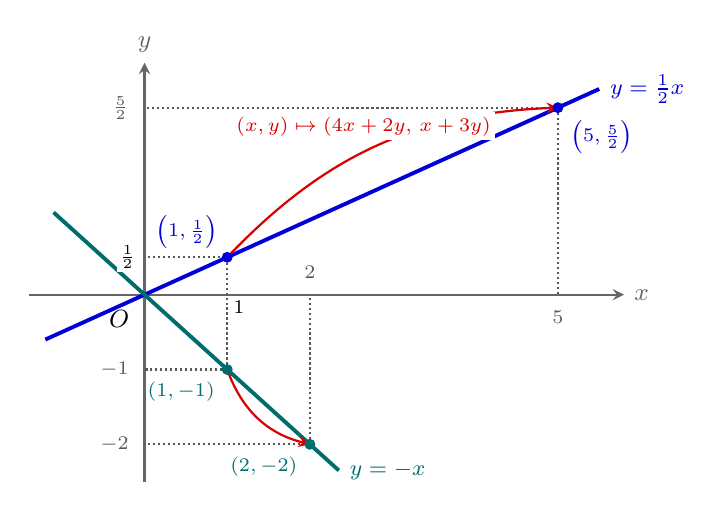
\begin{tikzpicture}[x=1.05cm, y=0.95cm, >=stealth, every node/.style={font=\small}]
    \coordinate (O) at (0, 0);
    \coordinate (P1) at (1, 0.5);
    \coordinate (P1p) at (5, 2.5);
    \coordinate (P2) at (1, -1);
    \coordinate (P2p) at (2, -2);

    % 座標軸
    \draw[->, thick, gray!80!black] (-1.4, 0) -- (5.8, 0) node[right] {$x$};
    \draw[->, thick, gray!80!black] (0, -2.5) -- (0, 3.1) node[above] {$y$};
    \node[below left=2pt] at (O) {$O$};

    % 不変直線 y = (1/2)x と y = -x
    \draw[line width=1.4pt, blue!85!black] (-1.2, -0.6) -- (5.5, 2.75)
    node[right, font=\footnotesize] {$y=\frac{1}{2}x$};
    \draw[line width=1.4pt, teal!85!black] (-1.1, 1.1) -- (2.35, -2.35)
    node[right, font=\footnotesize] {$y=-x$};

    % 座標軸への垂線（点線）
    \draw[densely dotted, thick, gray!70!black] (P2) -- (1, 0) -- (P1) -- (0, 0.5);
    \draw[densely dotted, thick, gray!70!black] (P1p) -- (5, 0) node[below=2pt, font=\scriptsize] {$5$};
    \draw[densely dotted, thick, gray!70!black] (P1p) -- (0, 2.5) node[left=2pt, font=\scriptsize] {$\frac{5}{2}$};
    \draw[densely dotted, thick, gray!70!black] (P2) -- (0, -1) node[left=2pt, font=\scriptsize] {$-1$};
    \draw[densely dotted, thick, gray!70!black] (P2p) -- (2, 0) node[above=2pt, font=\scriptsize] {$2$};
    \draw[densely dotted, thick, gray!70!black] (P2p) -- (0, -2) node[left=2pt, font=\scriptsize] {$-2$};
    \node[below right=1pt, font=\scriptsize, fill=white, inner sep=1pt] at (1, 0) {$1$};
    \node[left=2pt, font=\scriptsize, fill=white, inner sep=1pt] at (0, 0.5) {$\frac{1}{2}$};

    % 写像による移動の矢印
    \draw[->, thick, red!85!black] (P1) to[bend left=22]
    node[pos=0.46, above=4pt, font=\scriptsize, fill=white, inner sep=1.5pt] {$(x,y)\mapsto(4x+2y,\,x+3y)$} (P1p);
    \draw[->, thick, red!85!black] (P2) to[bend right=28] (P2p);

    % 点のプロットとラベル
    \node[circle, fill=blue!85!black, inner sep=1.4pt] at (P1) {};
    \node[above left=2pt, font=\scriptsize, blue!85!black, fill=white, inner sep=1pt] at (P1) {$\left(1,\frac{1}{2}\right)$};
    \node[circle, fill=blue!85!black, inner sep=1.4pt] at (P1p) {};
    \node[below right=1pt, font=\scriptsize, blue!85!black] at (P1p) {$\left(5,\frac{5}{2}\right)$};

    \node[circle, fill=teal!85!black, inner sep=1.4pt] at (P2) {};
    \node[below left=1pt, font=\scriptsize, teal!85!black] at (P2) {$(1,-1)$};
    \node[circle, fill=teal!85!black, inner sep=1.4pt] at (P2p) {};
    \node[below left=1pt, font=\scriptsize, teal!85!black] at (P2p) {$(2,-2)$};
  \end{tikzpicture}
  \caption{変換 $(x,y)\mapsto(4x+2y,\,x+3y)$ で不変な直線 $y=\dfrac{1}{2}x$ と $y=-x$}
  \label{fig:invariant_lines}
\end{figure}

まず，$l$が$y$軸平行な時を考える．この時は$l:x=\text{const.}$となるから，題意より
\begin{align}
  \forall y,x=4x+2y\Longleftrightarrow \forall y,3x+2y=0
\end{align}
となって矛盾する．
故に$l$は$y$軸平行ではなく，$a,b\in\mathbb{R}$に対して$y=f(x)=ax+b$とおける．
よって任意の$x$に対し
\begin{align}
  &f(4x+2y)=x+3y \nonumber\\
  \Longleftrightarrow &x+3(ax+b)=a(4x+2(ax+b))+b \nonumber\\
  \Longleftrightarrow &(3a+1)x+3b=(2a^2+4a)x+(2ab+b) \label{eq:1}
\end{align}
が成り立つ．つまり\cref{eq:1}が$x$についての恒等式なので
\begin{align}
  \left\{
    \begin{array}{l}
      3a+1=2a^2+4a \\
      3b=2ab+b
    \end{array}
    \right.     \\
    \Longleftrightarrow
    (a,b)=\left(\dfrac{1}{2},0\right),(-1,0)
  \end{align}
  である．従って求めるのは$y=-x$と$y=\dfrac{1}{2}x$である．$\cdots$(答)
  \newpage
  \end{document}
